\section{Termes atypiques}
  Pour identifier les termes atypiques, nous avons réutilisé le code vu précédemment pour obtenir l'équilibre des modalités.
  De cette manière, nous pouvons par exemple identifier que les départs de nuit sont peu fréquents. [fig:\ref{fig:DepTime}]

\begin{figure}[H]
  \centering
  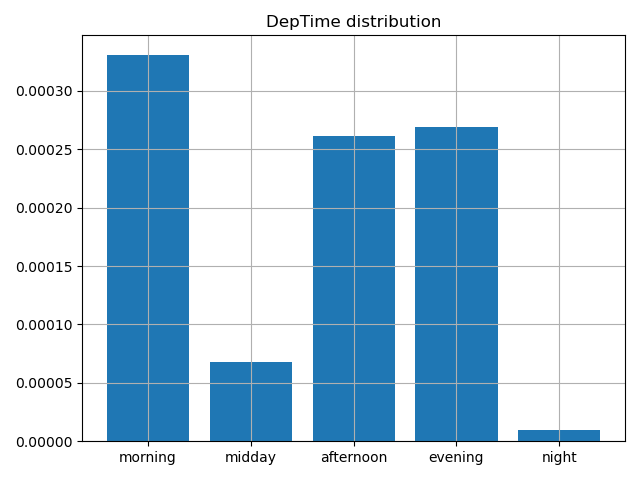
\includegraphics[scale=1]{images/DepTime_distribution.png}
  \caption{}
  \label{fig:DepTime}
\end{figure}

